% !TEX root = ../../main.tex
\section{Watershed Methods}\label{sec:rw_watershed_methods}

The watershed is a powerful tool for image segmentation.
It has been used for image segmentation since the work of
\citet{beucher_1979_workshop}.
The literature on watersheds is huge an 
a lot of definitions and algorithms exist
\citep{vinent_1991_pami,beuchner_1994_waterfall,najman_1994_sp,
roerdink_2000_finf,bertrand_2005_jmiv,cousty_2009_pami,
meyer_2012_corr,meyer_2012_corr2}.
A great overview  of the history of watersheds 
is given in the work of \citet{meyer_2012_corr}.
Recent watershed algorithms are discussed in \citep{meyer_2012_corr2}.

The watershed algorithm can be often described with the following  \emph{water flooding} analogy:
A grayscale  image can be interpreted as hight map (see \cref{fig:ws_2d_map}, \cref{fig:ws_2d_map3d}).
The water level is raised as shown in \crefrange{fig:ws_a}{fig:ws_f}.
A watershed is wherever the water of two adjacent valleys is meeting (see \cref{fig:ws_e},\cref{fig:ws_f} and \cref{fig:ws_2d_lines}).


An image may be interpreted as a node weighted graph,where the node weights
are given by the pixels gray value.
Watershed can also be applied to edge weighted graphs, where the nodes are unweighted 
and the edges connecting neighboring nodes encode the height between the pass points of two valleys.
\citet{meyer_2012_corr2} showed the relations between node and edge weighted watersheds. 





% watersheds illustrated
\begin{figure}[H]
    \centering
    \subfloat[1d Image Data]{ \label{fig:ws_a}
        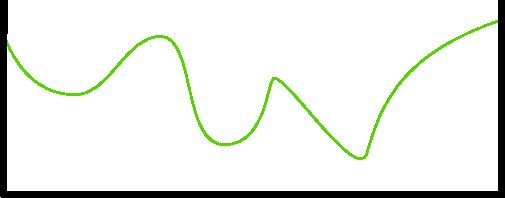
\includegraphics[width=0.25\textwidth]{fig/ws_no_no.pdf}
    }
    \hspace{0.5cm}
    \subfloat[Local minima]{  \label{fig:ws_b}
        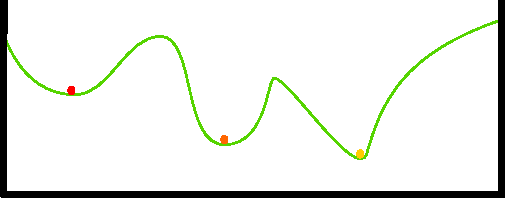
\includegraphics[width=0.25\textwidth]{fig/ws_no.pdf}
    }
    \hspace{0.5cm}
    \subfloat[flooding starts]{  \label{fig:ws_c}
        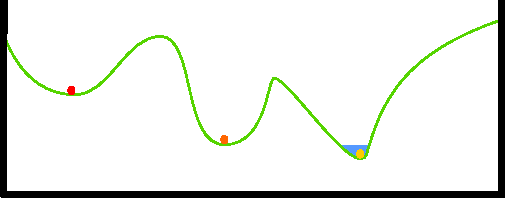
\includegraphics[width=0.25\textwidth]{fig/ws3.pdf}
    }
    \\
    \subfloat[flooding]{  \label{fig:ws_d}
        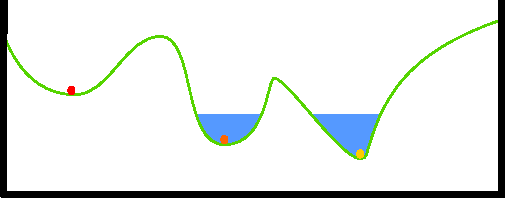
\includegraphics[width=0.25\textwidth]{fig/ws2.pdf}
    }
    \hspace{0.5cm}
    \subfloat[watershed 1]{  \label{fig:ws_e}
        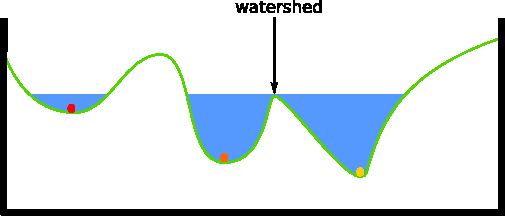
\includegraphics[width=0.25\textwidth]{fig/ws1.pdf}
    }
    \hspace{0.5cm}
    \subfloat[watershed 2]{ \label{fig:ws_f}
        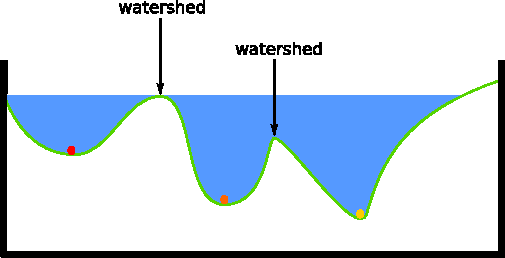
\includegraphics[width=0.25\textwidth]{fig/ws0.pdf}
    }
    \\ % 2D Watersheds
    \subfloat[$ $]{ \label{fig:ws_2d_map}
        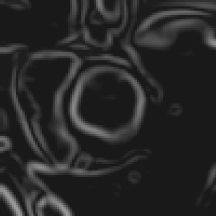
\includegraphics[height=0.26\textwidth]{fig/ws2d0.png}
    }
    \hspace{0.1cm}
    \subfloat[$ $]{ \label{fig:ws_2d_map3d}
        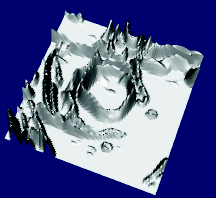
\includegraphics[height=0.26\textwidth]{fig/ws2d1.png} 
    }
    \hspace{0.1cm}
    \subfloat[$ $]{ \label{fig:ws_2d_lines}
        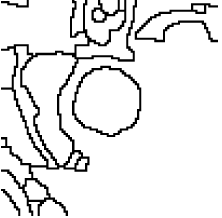
\includegraphics[height=0.26\textwidth]{fig/ws2d2.png}
    }

    \addtocontents{lof}{%
        \vspace{1cm}
        \protect\centerline{%
            \protect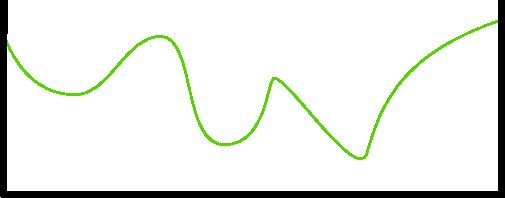
\includegraphics[width=.075\linewidth]{fig/ws_no_no.pdf}  \hspace{0.2cm}
            \protect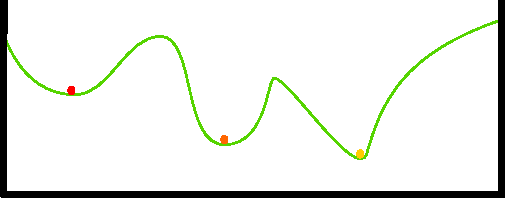
\includegraphics[width=.075\linewidth]{fig/ws_no.pdf}\hspace{0.2cm}
            \protect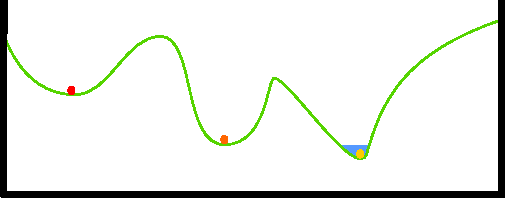
\includegraphics[width=.075\linewidth]{fig/ws3.pdf} 
        }%
        \vspace{0.2cm}
        \protect\centerline{%
            \protect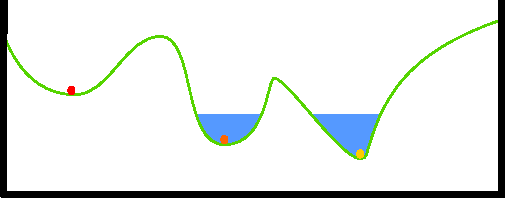
\includegraphics[width=.075\linewidth]{fig/ws2.pdf}  \hspace{0.2cm}
            \protect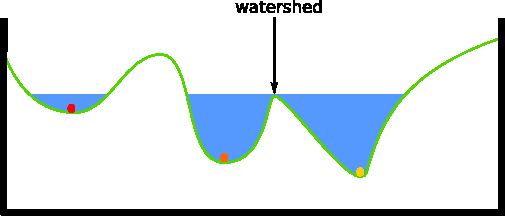
\includegraphics[width=.075\linewidth]{fig/ws1.pdf} \hspace{0.2cm}
            \protect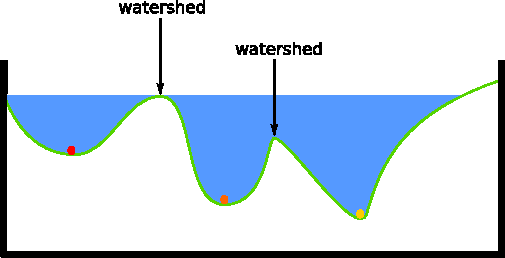
\includegraphics[width=.075\linewidth]{fig/ws0.pdf}%
        }%
        \vspace{0.2cm}
        \protect\centerline{%
            \protect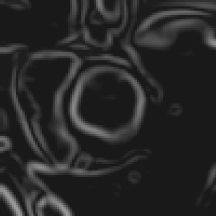
\includegraphics[height=.075\linewidth]{fig/ws2d0.png}  \hspace{0.2cm}
            \protect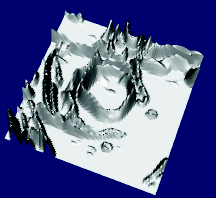
\includegraphics[height=.075\linewidth]{fig/ws2d1.png} \hspace{0.2cm}
            \protect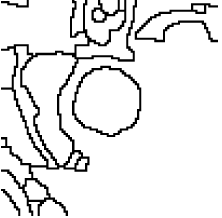
\includegraphics[height=.075\linewidth]{fig/ws2d2.png}%
        }%
    }%
    \caption[Illustration of watershed flooding process]{ 
        Illustration of watershed flooding process.
        The water level raises, and the watersheds are at the positions where water from different catchment basins is meeting.
        \Cref{fig:ws_2d_map} to \cref{fig:ws_2d_lines} have been taken from \citep{wiki_watersheds}.
    } \label{fig:watersheds_1d}
\end{figure}







\citet{couprie_2011_pami} proposed an algorithm, \emph{power-watershed}, a generalization of \citep{ boykov_2001_pami,vinent_1991_pami,najman_1994_sp,roerdink_2000_finf,bertrand_2005_jmiv,sinop_2007_iccv,cousty_2009_pami}.

They define the following model:
\begin{align}\label{eq:power_watershed}
\min_x \sum_{e_{ij} \in E}  w_{ip}^p |x_i-x_j|^q + \sum_{v_i } w_{Fi}^p |x_i|^q + \sum_{v_i } w_{Bi}^p |x_i-1|^q \\
s.t. \hspace{0.35cm} x(F)=1, \hspace{0.5cm} x(B)=0
\end{align}

Where $w_{ip}$ are edge weights and $w_{Fi}^p$ and $w_{Bi}^p$ are unaries weights
for foreground and background.

Setting $p$ to 1 will lead to the methods proposed by \citet{sinop_2007_iccv}.
\Citet{allene_icv_2010} pointed out when $p=1$ and $q \rightarrow \infty$, solving
\cref{eq:power_watershed} is equivalent to applying a minimum spanning forest algorithm.
\Cref{tab:power_ws} gives an overview how different choices $p$ and $q$ lead
to different well known segmentation methods, and to a new method, named \emph{power watershed}.

\begin{table}
    \begin{center}
    \begin{tabular}{|l|l|l|l|} \hline
    \backslashbox{q}{p}        & 0                              & finite & $\infty$              \\ \hline
    1           & -      & Graph cuts        & Power watershed           \\ \hline 
    2           & L2 norm Voronoi           & Random Walker     & Power watershed           \\ \hline 
    $\infty$    & L1 norm Voronoi           & L1 norm Voronoi   & Shortest Path Forest      \\ \hline 
    \end{tabular}
    \end{center}
    \caption{ \label{tab:power_ws}
        Power watershed parameterization: Different choices of parameters
        p and q lead to different segmentation methods.
        This table is identical to the table showed in \citet{couprie_2011_pami}.
    }
\end{table}


A drawback of the watershed method is water leaking to small ``holes'' in the height map / gradient image.
To overcome this weakness, 
\citet{meyer_2002_moprh}  proposed a flooding scheme with viscous mercury like
liquids.
This idea has been generalized to different viscous fluids in \citep{vachier_2005_jmiv}. 



\citet{straehle_2011_miccai} proposed a watershed based method for interactive segmentation
of neural volume electron  microscopy images.
They show how a background prior be be efficiently integrated into watersheds,
and that this prior is beneficial for neuro data.
In addition \citet{straehle_2012_cvpr} proposed an uncertainty estimator for
guided interactive segmentation based on watersheds.

\phantomsection
\label{sec:rw_waterfall}

Edge and node weighted watersheds on graphs can be applied recursively, since
the result of a watershed transformation itself is a more corsair graph.
This leads to a hierarchy of nested segmentation.
This transformation is called \emph{waterfall transformation} \cite{beuchner_1994_waterfall} and
the hierarchy is called \emph{waterfall hierarchy}.

\Citet{najman_1994_sp} showed, that there is a
strong connection between any hierarchical segmentations
and watersheds.
They prove that there exists a bijection between
the set of ultrametric watersheds\citep{najman_2010_corr} and the set of hierarchical segmentations.

